In figure \ref{fig:romc_overview} we present an overview of our
implementation; one may interpret figure~\ref{fig:romc_overview} as a
depiction of the main class of our implementation, called
(\pinline{ROMC}), while the entities inside the green and blue
ellipses are the main functions of the class. Following the common
naming principles, the methods starting with an underscore (green
ellipses) represent internal (private) functions and are not meant to
be used by a user, whereas the rest of the methods (blue ellipses) are
the functionalities the user interacts with. As mentioned before, the
implementation favours extensibility; the building blocks that compose
the method have been designed in an isolated fashion so that a
practitioner may replace them without the method to collapse.

Figure \ref{fig:romc_overview} groups the ROMC implementation into the
training, the inference and the evaluation part, following the
arrangement used in the algorithmic presentation (section
\ref{subsec:romc-algorithmic}). The training part includes all the
steps until the computation of the proposal regions; sampling the
nuisance variables, defining the optimisation problems, solving them,
constructing the regions and fitting local surrogate models. The
inference part comprises of evaluating the unnormalised posterior (and
the normalised one, in low-dimensional cases), sampling and computing
an expectation. Moreover, the ROMC implementation provides some
utilities for inspecting the training process, such as plotting the
histogram of the distances
$d^*_i = g_i(\theta_i^*), \: \forall i \in \{1, \ldots, n_1 \}$ after
solving the optimisation problems and visualising the constructed
bounding box\footnote{if the parametric space is up to $2D$}. Finally,
two functionalities for evaluating the inference are implemented; (a)
computing the Effective Sample Size (ESS) of the weighted samples and
(b) measuring the divergence between the approximate posterior the
ground-truth, if the latter is available.\footnote{Normally, the
  ground-truth posterior is not available; that is the meaning of
  performing the inference!  Though this functionality is useful in
  cases where the posterior can be computed numerically or with an
  alternative method (i.e.\ ABC Rejection Sampling) and we would like
  to measure the discrepancy between the two approximations.}


\subsubsection*{Simple 1D example}

For illustrating the functionalities we choose as running
example the following model, introduced by~\autocite{Ikonomov2019},

\begin{gather} \label{eq:1D_example}
  p(\theta) = \mathcal{U}(\theta;-2.5,2.5)\\
  p(y|\theta) = 
  \left\{
    \begin{array}{ll}
      \theta^4 + u & \mbox{if } \theta \in [-0.5, 0.5] \\
      |\theta| - c + u & \mbox{otherwise} 
    \end{array} \right.\\
  u \sim \mathcal{N}(0,1)
\end{gather}

\noindent

In the model \eqref{eq:1D_example}, the prior is the uniform
distribution in the range $[-2.5, 2.5]$ and the likelihood a Gaussian
distribution. There is only one observation $y_0 = 0$. The inference
in this particular example can be performed quite easily, without
icorporating a likelihood-free inference approach. Ee can exploit this
fact for validating the accuracy of our implementation. The
ground-truth posterior, approximated computationally, is shown in
figure \ref{fig:example_gt}.

\begin{figure}[h]
    \begin{center}
      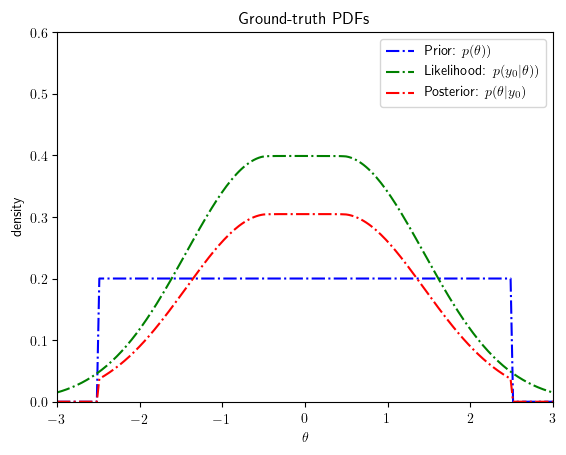
\includegraphics[width=0.5\textwidth]{./Thesis/images/chapter3/example_gt.png}
    \end{center}
  \caption[Ground-truth posterior distribution of the simple 1D example.]{Ground-truth posterior distribution of the simple 1D example.}
  \label{fig:example_gt}
\end{figure}

\subsubsection*{ELFI code for modelling the example}

In the following code snippet, we code the model at \textit{ELFI} and
we initialise the ROMC inference method. We observe that the
initialisation of the ROMC inference method is quite intuitive; we
just pass the final (distance) node of the simulator as argument, as
in all $\textit{ELFI}$ inference methods. The argument
\pinline{bounds}, although optional, is important for many
functionalities (e.g. approximating the partition function, setting
the bounds of the Bayesian optimisation etc.) so it is recommended to
be passed.

\begin{pythoncode}
  import elfi
  import scipy.stats as ss
  import numpy as np
  
  def simulator(t1, batch_size=1,random_state=None):
      if t1 < -0.5:
          y = ss.norm(loc=-t1-c, scale=1).rvs(random_state=random_state)
      elif t1 <= 0.5:
          y = ss.norm(loc=t1**4, scale=1).rvs(random_state=random_state)
      else:
          y = ss.norm(loc=t1-c, scale=1).rvs(random_state=random_state)
      return y

  # observation
  y = 0
      
  # Elfi graph    
  t1 = elfi.Prior('uniform', -2.5, 5)
  sim = elfi.Simulator(simulator, t1, observed=y)
  d = elfi.Distance('euclidean', sim)

  # Define ROMC inference method
  bounds = [(-2.5, 2.5)]
  romc = elfi.ROMC(d, bounds=bounds)
\end{pythoncode}


\begin{figure}[!ht]
    \begin{center}
      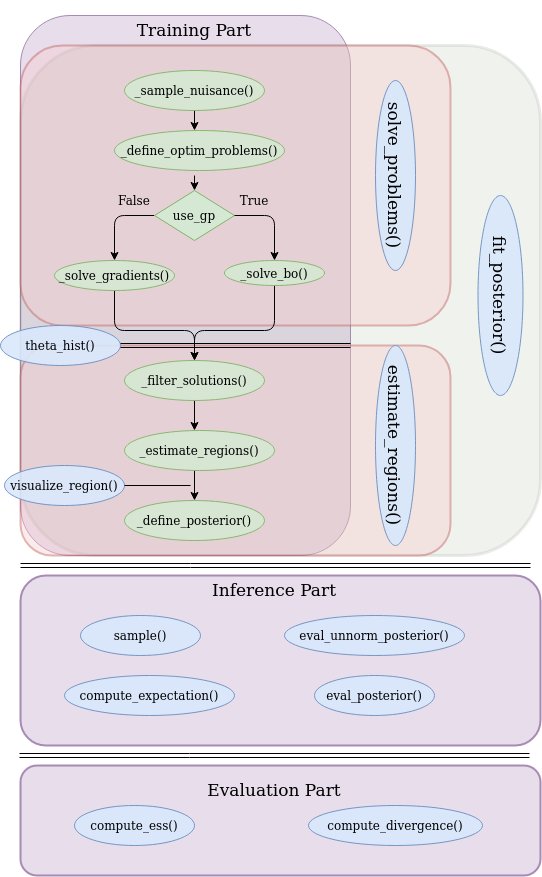
\includegraphics[width=0.8\textwidth]{./Thesis/graphs/ROMC.png}
    \end{center}
    \caption[Overview of the ROMC implementation.]{Overview of the ROMC implementation. The training part
      follows a sequential pattern; the functions in the green
      ellipses must be called in a sequential fashion for completing
      the training part and define the posterior distribution. The
      functions in blue ellipses are the functionalities provided to
      the user.}
    \label{fig:romc_overview}
\end{figure}

  